\documentclass{beamer}
%Information to be included in the title page:
\usetheme{Boadilla}
\definecolor{MITRed}{RGB}{163,31,52}
\definecolor{MITGray}{RGB}{138,139,140}
\usecolortheme[named=MITRed]{structure}

\setbeamertemplate{navigationsymbols}{}
\setbeamertemplate{headline}{\hfill
\includegraphics[width=1.5cm]{./MIT-logo-red-gray.png}\hspace{0.4cm}\vspace{-1.2cm}}
\beamertemplatenavigationsymbolsempty
\setbeamertemplate{blocks}[default]
\setbeamercolor{item projected}{bg=MITGray}

\begin{document}
	\title[]{Label-Aware Neural Tangent Kernel}
	% \subtitle{Chen et al. (2020)}
	\author[Suyeol Yun]{Suyeol Yun}
	% \institute[MIT]{6.S088}
	% \date{Feb 3, 2023}
	\frame{\titlepage}
	\section{Background}

	\begin{frame}{Label-Aware Neural Tangent Kernel}
		\centering	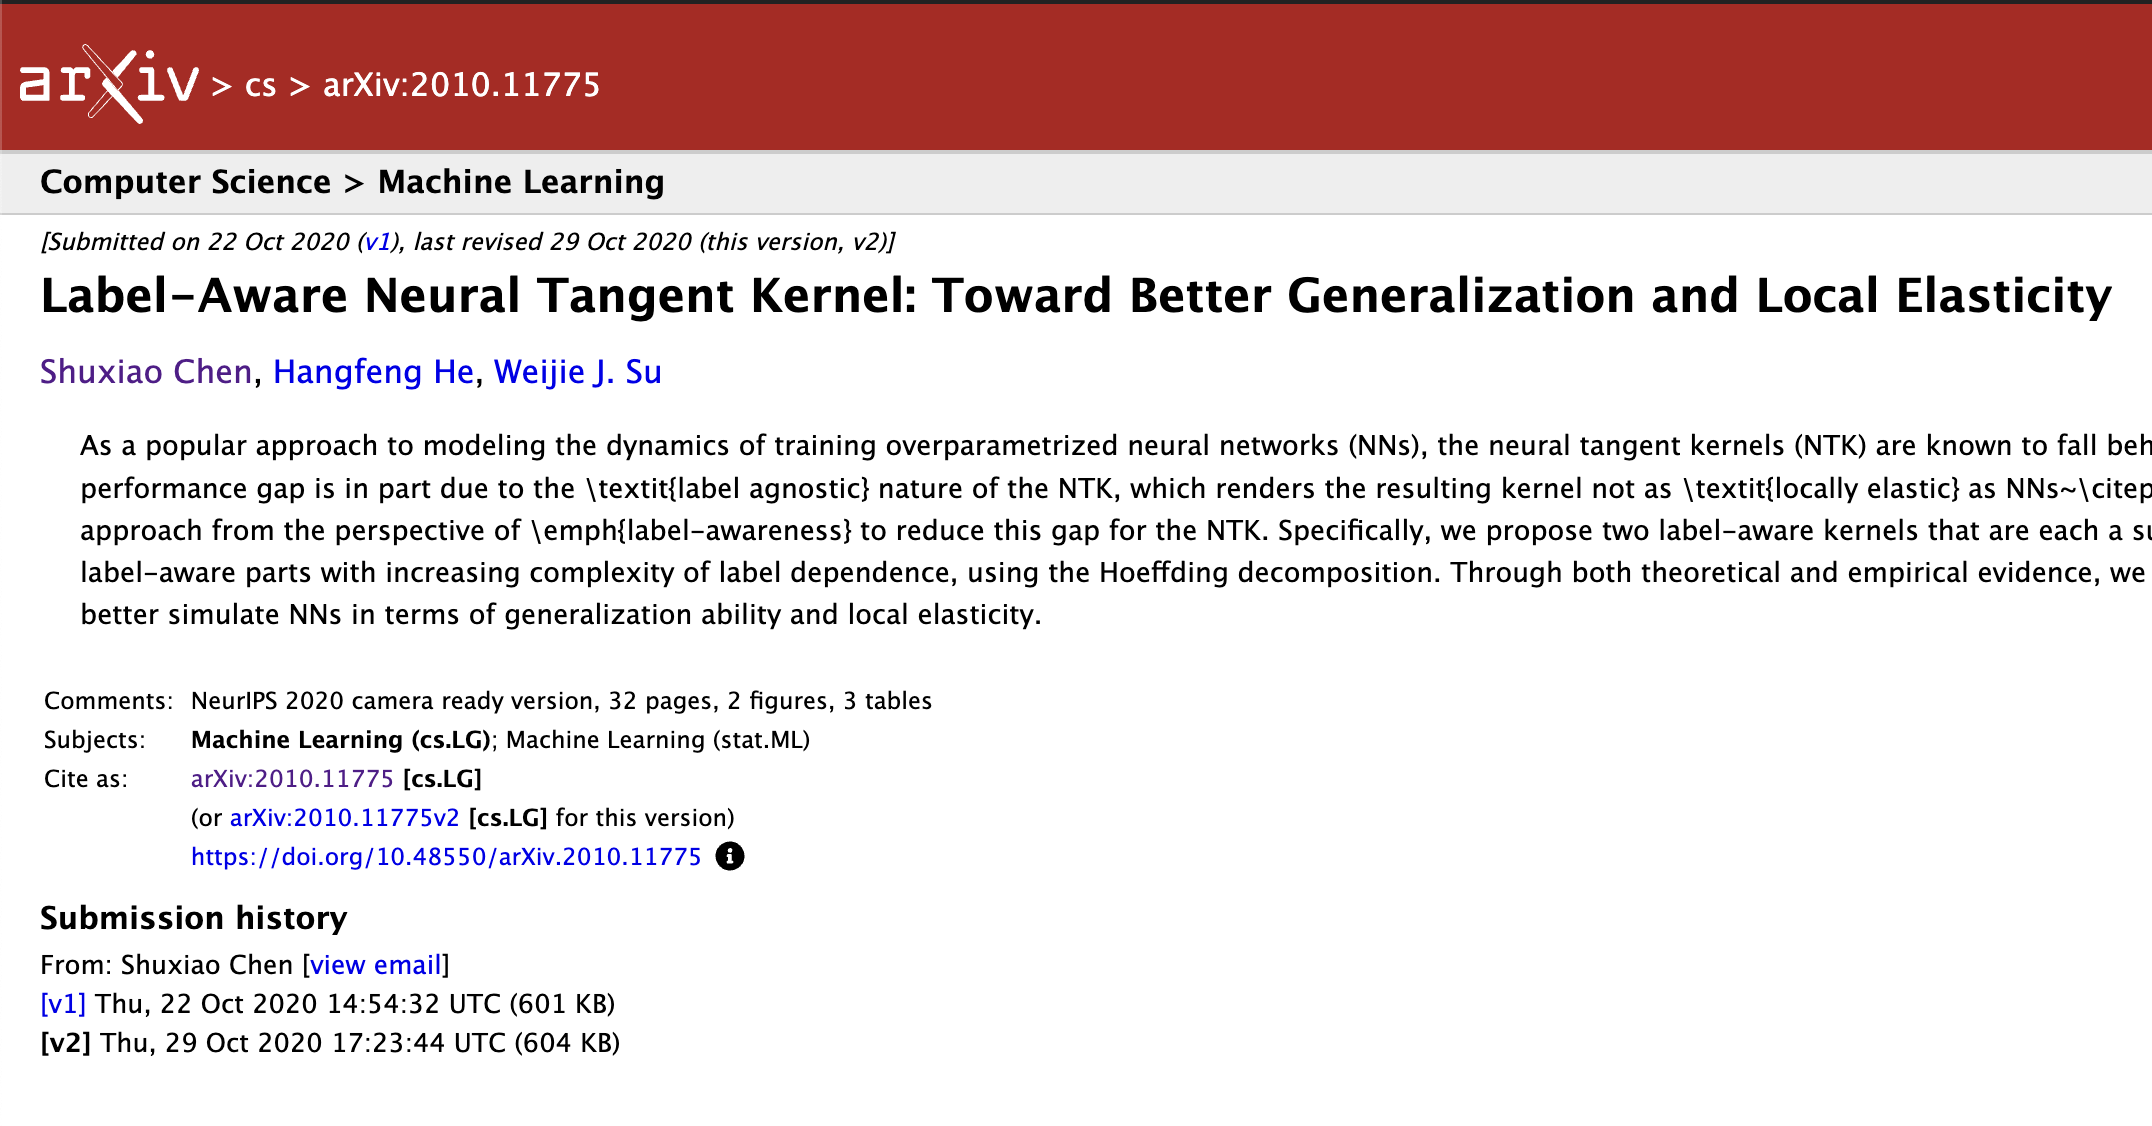
\includegraphics[scale=0.3]{./images/arxiv2.png}
		Chen et al. (Neurips 2020)
	\end{frame}

	\begin{frame}{Motivation}
		\begin{itemize}
			\item How to explain \textit{performance gap} between NTK and real-world NN?
			\item Arora (2019)
		\end{itemize}
		\centering	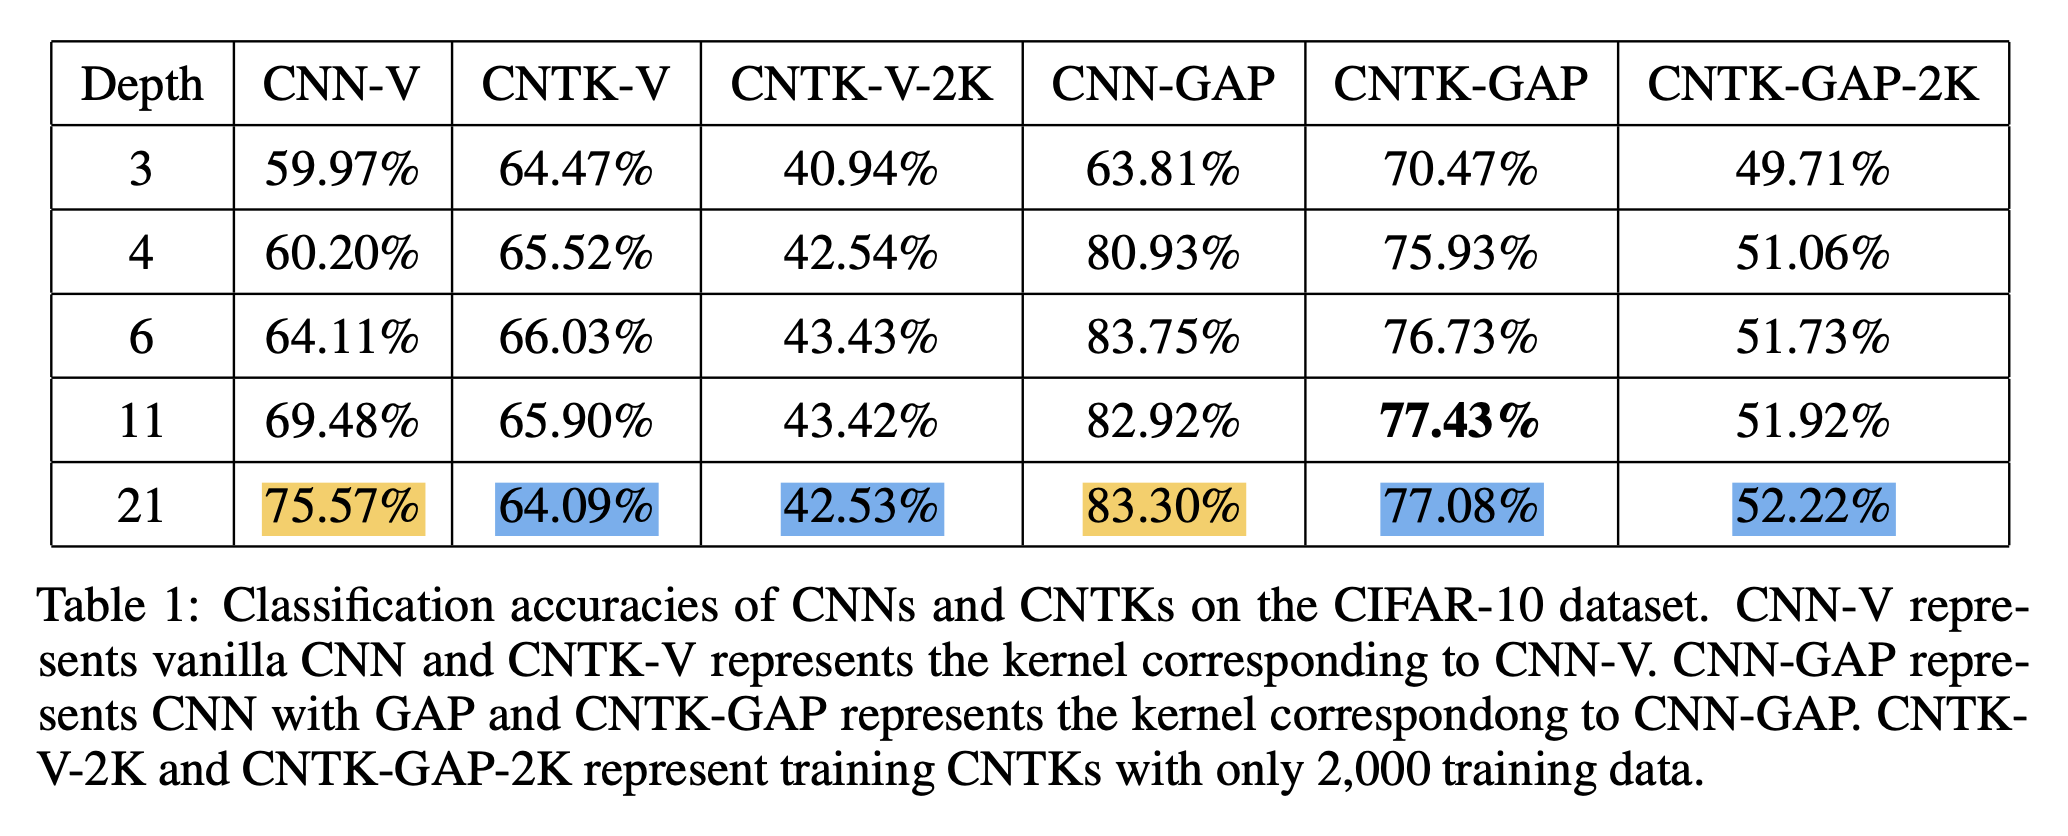
\includegraphics[scale=0.325]{./images/perfgap.png}
	\end{frame}

	\begin{frame}{Label-agnostic vs. Label-aware}
		% 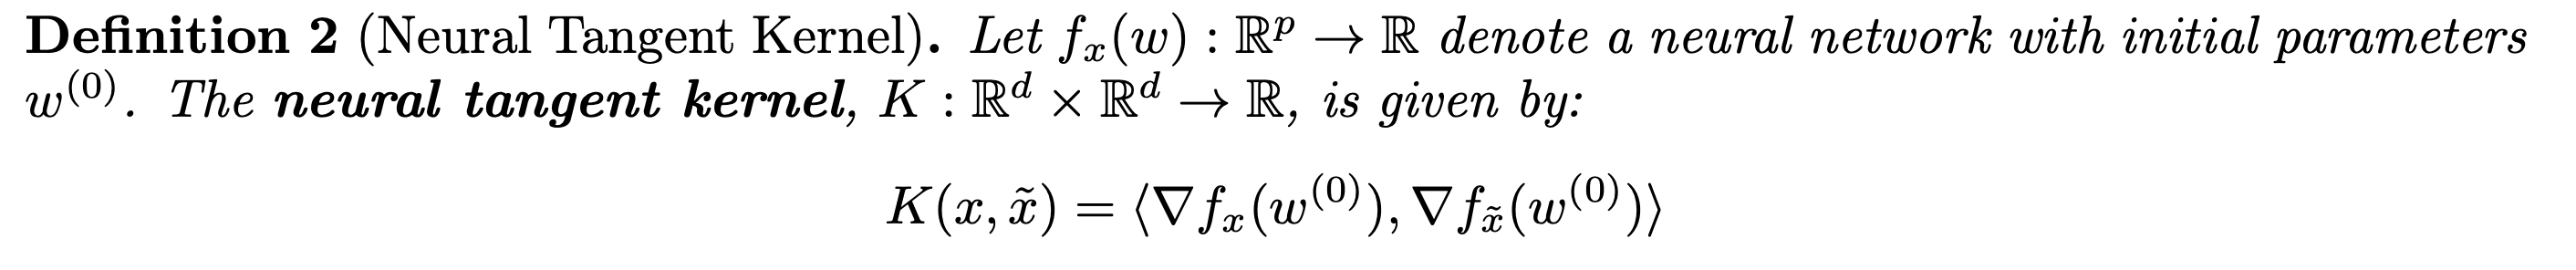
\includegraphics[scale=0.25]{./images/ntkdef.png}

		\begin{itemize}
			\item NN is label-aware while NTK is label-agnostic
			\item NTK construction is independent of the labels\footnote{Remind that NTK is soley a function of a network architecture.}
			$$K_{NTK}(x, \tilde{x})=\left\langle\nabla f_x\left(w^{(0)}\right), \nabla f_{\tilde{x}}\left(w^{(0)}\right)\right\rangle$$
			\item NN can be thought of \textit{label-aware} because trained parameter of NN depend on labels.
		\end{itemize}
	\end{frame}

	\begin{frame}{Label-aware NTK}
		\begin{itemize}
			\item Goal is to develop a label-aware NTK.
			% \begin{itemize}
			% \item Good feature map $\phi$ maps $x$ close to its label.
			\item \textit{Optimal} feature map $\phi^{\star}(x_i)=y_i$
			\item \textit{Optimal} kernel  
			% \end{itemize}
			$
			K^{\star}\left(x_i, x_j\right)=\left\langle\phi^{\star}(x_i), \phi^{\star}(x_j)\right\rangle = y_i y_j
			$
			\item But we don't know $y_\alpha$ and $y_\beta$ for test cases. So design estimator of $y_\alpha y_\beta$ and augment it to NTK.
			$$K_{\text{LA-NTK}}(x_i, x_j)= K_{NTK} + \lambda \mathcal{Z}\left(x_i, x_j, \mathcal{D}\right)$$
			\quad \quad where $\mathcal{Z}\left(x_i, x_j, \mathcal{D}\right)=y^{\top} \mathbf{M}\left(x_i, x_j, X\right) y$ which is a linear regression model to estimate $y_iy_j$ for given $(x_i, x_j)$.
		\end{itemize}
	\end{frame}

	\begin{frame}{Performance of Label-aware NTK}
		\centering	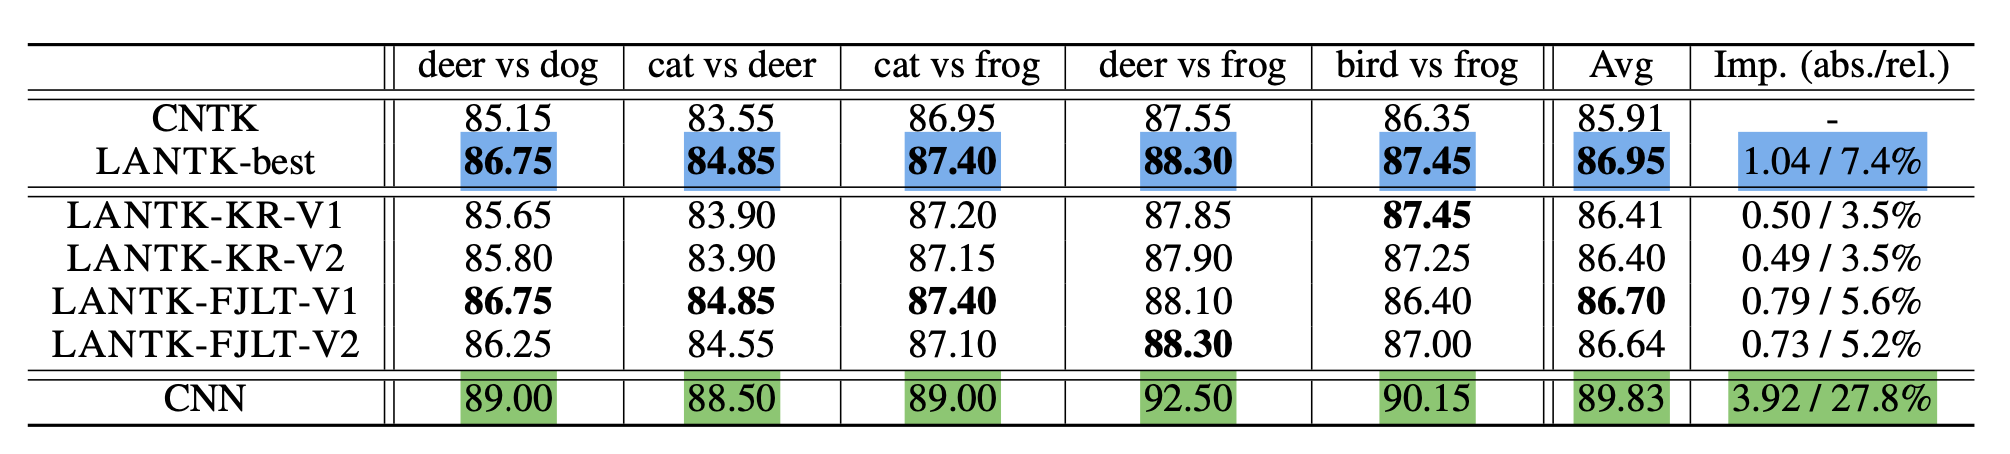
\includegraphics[scale=0.35]{./images/perfrpt.png}\footnote{
			``... this is a theoretically motivated work, so I am not concerned about the size of the empirical improvements.''
		}
	\end{frame}

	\begin{frame}{Further thoughts}
		\begin{itemize}
			\item What else remains to explain performance gap between NTK and NN?
			\begin{itemize}
				\item Is label-agnostic asepct of NTK sufficient to explain performance gap?
			\end{itemize}
			\item The reason of underperformance compared to CNN maybe due to the limited expressivity of $\mathcal{Z}$ used in the paper which estimates $y_iy_j$ given $(x_i, x_j)$.
			\item Will there be anyway to derive this $\mathcal{Z}$ part analytically as a function of network architecture as well as we did in derivation of NTK?
		\end{itemize}
	\end{frame}

	\begin{frame}{References}
		\begin{itemize}
			\item Sanjeev Arora, Simon S Du, Wei Hu, Zhiyuan Li, Russ R Salakhutdinov, and Ruosong Wang. On exact computation with an infinitely wide neural net. In Advances in Neural Information Processing Systems, pp. 8139–8148, 2019a.
			\item Shuxiao Chen, Hangfeng He, Weijie J. Su:
			Label-Aware Neural Tangent Kernel: Toward Better Generalization and Local Elasticity. NeurIPS 2020
		\end{itemize}
	\end{frame}
\end{document}

